Motores de passo são distinguíveis principalmente pela sua característica construtiva principal, i.e., se são com relutância variável ou com ímã permanente, ou uma combinação de ambos.

Um motor de passo com relutância variável consiste em um rotor de ferro com múltiplos dentes e um estator com enrolamentos. Os polos ficam magnetizados quando os enrolamentos do estator são energizados com corrente DC. O mesmo será rotacionado quando os dentes do estator são atraídos para os pólos do estator energizado para o que o sistema tenha o circuito com menor relutância. 

\begin{figure}[ht!]
    \center 
    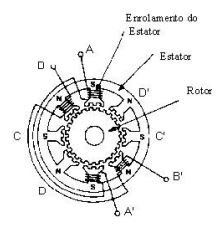
\includegraphics[scale=0.9]{imagens/f13}
    \caption{Motor de Relutância Variável.}
\end{figure}

Já motores de ímã permanente possuem seu rotor construído com ímãs permanentes e sem dentes. Os pólos magnetizados do rotor dão uma maior intensidade de fluxo magnético e portanto este motor terá uma melhor característica de torque. O mesmo tem baixo custo e baixa resolução. 

\begin{figure}[ht!]
    \center 
    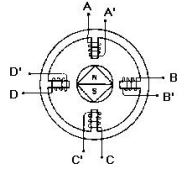
\includegraphics[scale=0.8]{imagens/f14}
    \caption{Motor de Ímã Permanente.}
    \end{figure}
\newpage

Os motores híbridos possuem um melhor desempenho em velocidade, torque e resolução de passo que os outros dois tipos. Eles são uma combinação dos motores de ímã permanente e de relutância variável tendo seu rotor com múltiplos dentes e um ímã permanente ao redor do eixo. 


\begin{figure}[ht!]
    \center 
    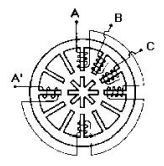
\includegraphics[scale=1]{imagens/f15}
    \caption{Motor Híbrido.}
\end{figure}

